% Created 2019-12-02 Mon 11:03
% Intended LaTeX compiler: pdflatex
\documentclass[11pt]{article}
\usepackage[utf8]{inputenc}
\usepackage[T1]{fontenc}
\usepackage{graphicx}
\usepackage{grffile}
\usepackage{longtable}
\usepackage{wrapfig}
\usepackage{rotating}
\usepackage[normalem]{ulem}
\usepackage{amsmath}
\usepackage{textcomp}
\usepackage{amssymb}
\usepackage{capt-of}
\usepackage{hyperref}
\author{Dhruv Dhamani}
\date{\today}
\title{Why my Project is pointless}
\hypersetup{
 pdfauthor={Dhruv Dhamani},
 pdftitle={Why my Project is pointless},
 pdfkeywords={},
 pdfsubject={},
 pdfcreator={Emacs 26.3 (Org mode 9.3)}, 
 pdflang={English}}
\begin{document}

\maketitle

\section{Intelligent Agent}
\label{sec:orgcdc4f13}
\begin{center}
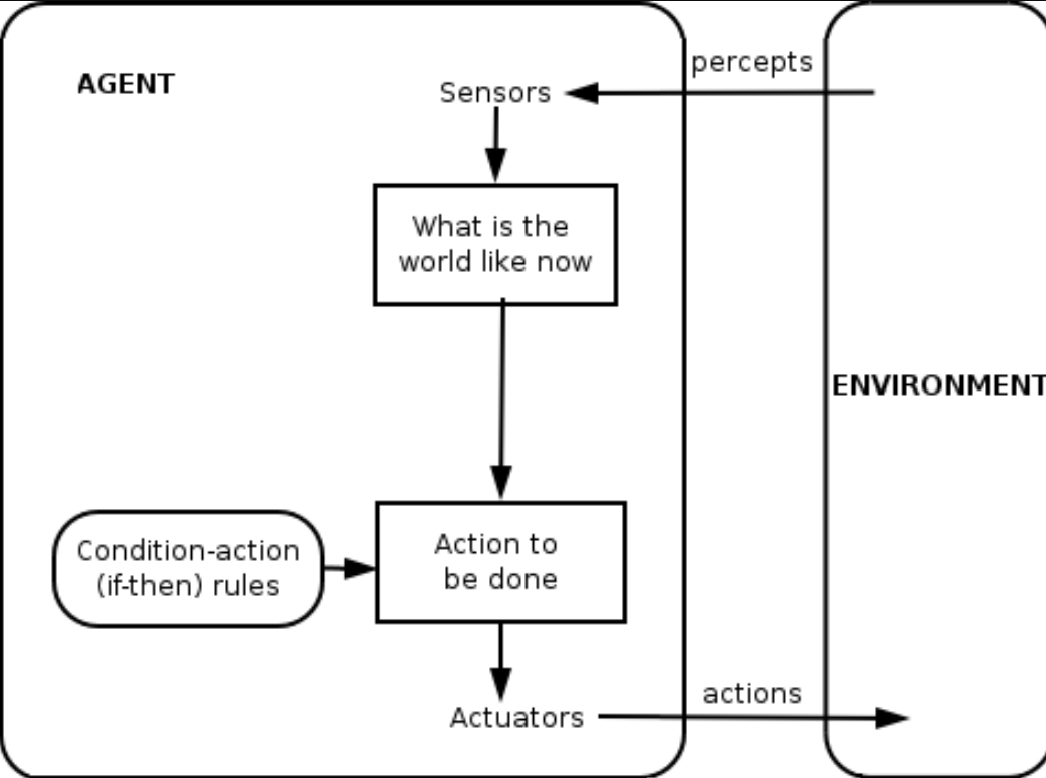
\includegraphics[width=.9\linewidth]{./ia.png}
\end{center}

\section{An example.}
\label{sec:org526a7c3}

\begin{itemize}
\item Book a spot for three at Maid-Rite Sandwich Shop in Antigua and Barbuda. I'll
book a table for you at [\ldots{}]
\item Book a spot for three at Maid-Rite Sandwich Shop in Antigua and Barbuda. Which
place? [\ldots{}]
\item Book a spot for three at Maid-Rite Sandwich Shop in Antigua and Barbuda. I'll
book a table for [\ldots{}]
\end{itemize}

\section{An example.}
\label{sec:orgcf6e38d}

\begin{itemize}
\item Book a spot for three at Maid-Rite Sandwich Shop in Antigua and Barbuda. I'll
book a table for you at \uline{Maid-Rite Sandwich}
\item Book a spot for three at Maid-Rite Sandwich Shop in Antigua and Barbuda. Which
place? \uline{Maid-Rite Sandwich}
\item Book a spot for three at Maid-Rite Sandwich Shop in Antigua and Barbuda. I'll
book a table for \uline{three}
\end{itemize}

\section{RoBERTa}
\label{sec:org491ad61}

RoBERTa iterates on BERT's pretraining procedure, including training the model longer, with bigger batches over more data; removing the next sentence prediction objective; training on longer sequences; and dynamically changing the masking pattern applied to the training data.


\section{RoBERTa}
\label{sec:org8edc141}

\begin{itemize}
\item Bi-directional masked language model.
\end{itemize}

\section{What I intended to do -}
\label{sec:orgae2a165}

\begin{itemize}
\item Book a spot for three at Eve's Pizzeria. Which place? \texttt{<mask>}
\end{itemize}

\section{What I intended to do -}
\label{sec:org7a027fc}
\begin{itemize}
\item Book a spot for three at Eve's Pizzeria. Which place? \texttt{<mask>}
\item Book a spot for three at Eve's Pizzeria. Which place? Eve's \texttt{<mask>}
\item Book a spot for three at Eve's Pizzeria. Which place? Eve's Pizzeria
\end{itemize}

\section{What actually happens -}
\label{sec:org5b1a3ca}


\begin{itemize}
\item <s> Book a spot for three at Eve's Pizzeria. Which place? </s>
\end{itemize}

\section{What actually happens -}
\label{sec:org53f04c3}
\begin{itemize}
\item <s> Book a spot for three at Eve's Pizzeria. Which place? Eve's </s></s>
\item <s> Book a spot for three at Eve's Pizzeria. Which place? Eve's </s></s></s></s></s></s></s></s>
\end{itemize}

\section{How to get it to work -}
\label{sec:orgaf19293}

\begin{itemize}
\item Don't use a birdirectional masked language model.
\item Examples of GPT2, a uni-directional transformer model trained for the same
task -
\begin{itemize}
\item add artist to All Out 70s . Where should I add ? All Out 70s
\item Give the current  book a three . What is the rating ? three
\item \url{https://colab.research.google.com/drive/1MGDjZDdgzxZtAI\_KO2yDEOkRmX3jj2LD}
\end{itemize}
\item Do not use dynamic masking, as the orignal paper did, instead mask only the
final answer.
\begin{itemize}
\item What the paper did -
\begin{itemize}
\item Book a \texttt{<mask>} for three \texttt{<mask>} Eve's Pizzeria. Which place? Eve's
Pizzeria.
\end{itemize}
\item Instead, do -
\begin{itemize}
\item Book a spot for three at Eve's Pizzeria. Which place? \texttt{<mask>
     <mask>}
\end{itemize}
\end{itemize}
\end{itemize}

\section{Any questions?}
\label{sec:org2a64843}
\end{document}
